\documentclass[sigconf,nonacm,10pt]{acmart}
\settopmatter{printacmref=false,printfolios=true}
\setcopyright{none}
\renewcommand\footnotetextcopyrightpermission[1]{}
\usepackage{amsmath,tabularx,array,enumitem,balance,tikz}
\geometry{a4paper,left=15mm,right=15mm,top=15mm,bottom=15mm}
\usetikzlibrary{arrows.meta,positioning,shapes.geometric}
\definecolor{CourseBlue}{HTML}{315EFB}
\definecolor{CourseTeal}{HTML}{14877D}
\definecolor{CourseInk}{HTML}{18324A}
\hypersetup{colorlinks=true,linkcolor=CourseBlue,citecolor=CourseTeal,urlcolor=CourseTeal}
\newcolumntype{Y}{>{\raggedright\arraybackslash}X}
\setlist{leftmargin=*,topsep=3pt,itemsep=2pt}
\newcommand{\CourseNumber}{COMSCI/ECON 206}
\newcommand{\CourseName}{Computational Microeconomics}
\newcommand{\CourseSession}{Autumn 2026 Session 1}
\newcommand{\Instructor}{Professor Luyao Zhang}
\newcommand{\TeamCode}{FP4}
\newcommand{\SymposiumSession}{D}
\newcommand{\GitHubLink}{\href{https://github.com/dku-comsci-econ206-Autumn2026/PS2-FP4-CapabilityTransfer}{\texttt{PS2-FP4-CapabilityTransfer}} (exact tested commit: \texttt{[FINAL-COMMIT]})}
\newcommand{\NotebookLink}{\texttt{k\_formula.ipynb}, \texttt{verify\_k.py}, and \texttt{code/distill\_sim.py} (seed 206) in the repository above}
\newcommand{\HuggingFaceLink}{Prize Rate Game: \href{https://huggingface.co/spaces/dku-comsci-econ206-2026/FP4_PS2}{\texttt{FP4\_PS2}} (Hugging Face Space)}
\newcommand{\PosterLink}{Root \texttt{README.md} embeds \texttt{poster/final-poster.png} and links \texttt{poster/final-poster.pdf}}
\newcommand{\coursemeta}{\noindent\textbf{Submission to:} \CourseNumber{} --- \CourseName.\\
\textbf{Course session:} \CourseSession. \textbf{Team:} \TeamCode. \textbf{Final week:} October 12 and 14, 2026.\\
\textbf{Course instructor:} \Instructor. \textbf{Assignment:} Final project revised research submission.\par\smallskip}
\title{Pay for Training, Not for Openness: Reward Design for Original and Distilled AI Models}
\author{Zhengjun He}
\affiliation{\institution{Duke Kunshan University}\city{Kunshan}\country{China}}
\email{zhengjun.he@dukekunshan.edu.cn}
\author{Yichen Shen}
\affiliation{\institution{Duke Kunshan University}\city{Kunshan}\country{China}}
\email{yichen.shen@dukekunshan.edu.cn}
\renewcommand{\shortauthors}{Team \TeamCode}

% The instructor is course metadata, not a paper author.
\newif\ifTeachingAnnotations
\TeachingAnnotationsfalse
% Visible, printable teaching notes. The original ACM text area is unchanged.
% Use main.tex for the clean submission and annotated.tex for guidance.
\ifTeachingAnnotations
\usepackage{eso-pic,tikz}
\usepackage[most]{tcolorbox}
\definecolor{AnnReplace}{HTML}{245BB4}
\definecolor{AnnConnect}{HTML}{08756C}
\definecolor{AnnDevelop}{HTML}{79469C}
\definecolor{AnnInk}{HTML}{21324A}
\definecolor{AnnRail}{HTML}{F4F6FA}
\definecolor{AnnLine}{HTML}{D4DCE7}
\newsavebox{\AnnRailBox}
\newcommand{\AnnNote}[4]{%
  \begin{tcolorbox}[enhanced,sharp corners,boxrule=0pt,frame hidden,
    colback=#2!5!white,borderline west={2pt}{0pt}{#2},
    left=7pt,right=7pt,top=5pt,bottom=5pt,before skip=6pt,after skip=0pt]
    \sffamily\fontsize{9.4}{11.8}\selectfont\color{AnnInk}\raggedright
    {\color{#2}\bfseries #1\quad #3}\par\vspace{2pt}#4
  \end{tcolorbox}}
\newcommand{\AnnPin}[4]{%
  \node[rounded corners=2bp,fill=#2,text=white,inner xsep=4bp,
    inner ysep=2.5bp,font=\sffamily\bfseries\fontsize{8}{9}\selectfont]
    at (#3,#4) {#1};}
\newcommand{\AnnPageTitle}{%
  \ifcase\value{page}\or
    Eight required parts\or
    Integrate evidence and impact\or
    Authorship and reproducibility\or
    Final week and release audit\or
    Add only the PS2 extension record\else
    Final release and evidence\fi}
\newcommand{\AnnPageNotes}{%
  \ifcase\value{page}\or\AnnNote{R}{AnnReplace}{Keep authorship accurate}{Replace title, team code, author names and emails. Keep the course, term and Professor Luyao Zhang as instructor metadata. Remove unused author slots.}

\AnnNote{C}{AnnConnect}{Preserve eight named parts}{Background, Motivation, Application Scenario, Research Question and Method begin the main paper. Results, Intellectual Merits and Practical Impacts continue on page 2.}

\AnnNote{D}{AnnDevelop}{Make the strategy inspectable}{Define players, strategies, payoffs, timing and information before selecting a solution concept. Connect game theory, social choice and mechanism design to a tested comparison.}

\AnnNote{R}{AnnReplace}{Retain the two A4 page limit}{Both main pages include metadata, principal diagram, captions and artifact links. Expanded diagrams and technical records can move to the appendices.}\or
    \AnnNote{D}{AnnDevelop}{Make the merits claim survive review}{Compare three verified closest papers. Annotate the model diagram to separate inherited foundations, distinct contribution and evidence.}

\AnnNote{C}{AnnConnect}{Put SDGs on the impact diagram}{Use official icons and target codes. Explain mechanism, stakeholders, indicator, baseline, evidence status, risk and safeguard.}

\AnnNote{D}{AnnDevelop}{Create a new roadmap diagram}{Give the next economics, CS and behavioral studies with question, method/data, possible collaborator, progress criterion and milestone.}

\AnnNote{R}{AnnReplace}{Use the final deadline}{Final project: Wednesday, October 21, 2026, 11:00 p.m. Asia/Shanghai. Upload paper PDF, source ZIP, poster PPTX and poster PDF.}\or\AnnNote{R}{AnnReplace}{Update contributions and credit}{Every named member needs a personal decision, inspectable output, verification and integration. BOTH paper and poster must contain these updated statements and FULL acknowledgments.}

\AnnNote{C}{AnnConnect}{Respond to all feedback sources}{Use instructor feedback, formal peer documents and in-class discussions. Record source/date, decision/reason, changed location, evidence or next test and responsible author.}

\AnnNote{D}{AnnDevelop}{Keep verification and disclosure}{Run the cited output from a fresh environment. Record exact versions, limitations, source licenses and bounded AI assistance. Retain the cumulative development record.}\or
    \AnnNote{C}{AnnConnect}{Connect final week activities}{Oct 12 stress-tests the claim through three papers and paired defense. Oct 14 challenges assumptions through self-tests, peer dialogue and symposium. Record the resulting research decision.}

\AnnNote{R}{AnnReplace}{Embed the actual poster}{Commit a readable PNG/JPG and the full PDF to GitHub. Embed the preview and link the PDF in ROOT README.md. An external poster link alone is insufficient.}

\AnnNote{D}{AnnDevelop}{Audit the synchronized release}{The paper, notebook/code, Space and poster must agree on question, assumptions, parameters, outputs, evidence status, version, contributions and credit. Verify all four uploads with every member.}\or\AnnNote{D5}{AnnDevelop}{Record the auction, not only the outcome}{%
State values or signals, prediction, bid, allocation, payment, stopping rule, utility, revenue, efficiency, behavioral observation, and revision for each treatment.}

\AnnNote{C5}{AnnConnect}{Check parity across three artifacts}{%
GitHub, Hugging Face, and the A0 poster must describe the same question, model, evidence status, result, and limits. The labels describe evidence perspectives, not fixed team roles.}

\AnnNote{D6}{AnnDevelop}{Use the symposium to revise}{%
Retain the September 28 poster and reviews. Record Keep, Revise, or Investigate decisions, rerun the affected check, and identify the exact September 30 change.}
\else
    \AnnNote{D}{AnnDevelop}{Return to the clean driver}{Use \texttt{main.tex} for submission. Recheck the two-page main limit and preserve supporting evidence in the appendices.}
  \fi}
\newcommand{\AnnPagePins}{%
  \ifcase\value{page}\or
    \AnnPin{R1}{AnnReplace}{31}{88}
    \AnnPin{R2}{AnnReplace}{31}{370}
    \AnnPin{C1}{AnnConnect}{31}{510}
    \AnnPin{D1}{AnnDevelop}{581}{400}
  \or
    \AnnPin{C2}{AnnConnect}{31}{94}
    \AnnPin{D2}{AnnDevelop}{31}{240}
    \AnnPin{R3}{AnnReplace}{581}{340}
  \or
    \AnnPin{R4}{AnnReplace}{31}{105}
    \AnnPin{D3}{AnnDevelop}{31}{390}
    \AnnPin{C3}{AnnConnect}{581}{240}
  \or
    \AnnPin{R5}{AnnReplace}{31}{92}
    \AnnPin{C4}{AnnConnect}{31}{260}
    \AnnPin{D4}{AnnDevelop}{31}{420}
  \or
    \AnnPin{D5}{AnnDevelop}{31}{92}
    \AnnPin{C5}{AnnConnect}{31}{310}
    \AnnPin{D6}{AnnDevelop}{581}{260}
  \fi}
\AddToHook{shipout/before}{\global\pdfpagewidth=912bp\relax}
\AddToShipoutPictureBG{\AtPageUpperLeft{%
  \begin{tikzpicture}[overlay,x=1bp,y=-1bp]
    \fill[AnnRail] (612,0) rectangle (912,842);
    \draw[AnnLine,line width=.6bp] (612,0)--(612,792);
  \end{tikzpicture}}}
\AddToShipoutPictureFG{\AtPageUpperLeft{%
  \savebox{\AnnRailBox}{\normalfont\begin{minipage}[t]{266bp}\AnnPageNotes\end{minipage}}
  \begin{tikzpicture}[overlay,x=1bp,y=-1bp]
    \AnnPagePins
    \node[anchor=north west,inner sep=0,text width=266bp] at (629,26) {%
      \sffamily\color{AnnInk}\fontsize{10}{12}\selectfont\raggedright
      {\fontsize{9}{11}\selectfont\bfseries FINAL PROJECT ANNOTATED COPY}\par\vspace{5pt}
      {\fontsize{15}{17}\selectfont\bfseries\AnnPageTitle}\par\vspace{7pt}
      {\fontsize{9}{11}\selectfont
      \textcolor{AnnReplace}{\textbf{R REPLACE}}\quad
      \textcolor{AnnConnect}{\textbf{C CONNECT}}\quad
      \textcolor{AnnDevelop}{\textbf{D DEVELOP}}}};
    \node[anchor=north west,inner sep=0] at (629,102) {\usebox{\AnnRailBox}};
    \node[anchor=north west,inner sep=0,text width=266bp] at (629,798) {%
      \sffamily\fontsize{8.4}{10.2}\selectfont\color{AnnInk}
      Guidance is scaffolding. Submit from \texttt{main.tex}.
      \textbf{\thepage/4}};
  \end{tikzpicture}}}
\fi


\begin{document}
\begin{teaserfigure}
\captionsetup{skip=8pt}
\centering
\resizebox{0.48\textwidth}{!}{%
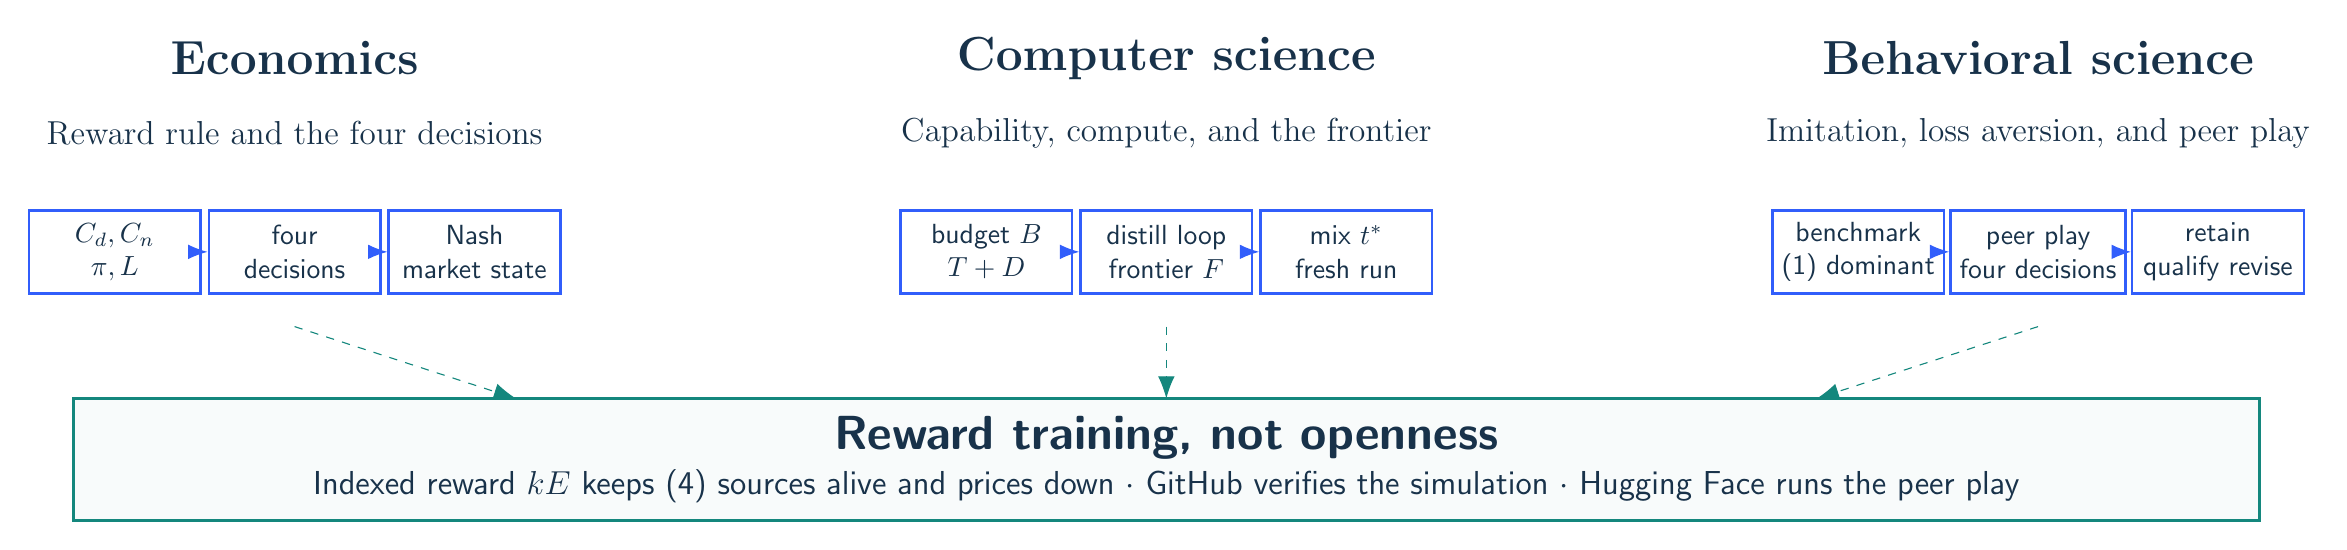
\begin{tikzpicture}[x=1pt,y=1pt,font=\sffamily,>=Latex]
\tikzset{
  heading/.style={font=\bfseries\fontsize{18}{20}\selectfont,text=CourseInk,align=center},
  label/.style={font=\fontsize{12}{14}\selectfont,text=CourseInk,align=center},
  mini/.style={draw=CourseBlue,line width=0.9pt,minimum width=62pt,minimum height=30pt,align=center,text=CourseInk,fill=white},
  synthesis/.style={draw=CourseTeal,line width=1.1pt,minimum width=790pt,minimum height=44pt,align=center,text=CourseInk,fill=CourseTeal!3}
}
\node[heading] at (140,190) {Economics};
\node[label] at (140,163) {Reward rule and the four decisions};
\node[mini] (e1) at (75,120) {$C_d,C_n$\\$\pi,L$};
\node[mini] (e2) at (140,120) {four\\decisions};
\node[mini] (e3) at (205,120) {Nash\\market state};
\draw[CourseBlue,-{Latex[length=7pt]}] (e1)--(e2);
\draw[CourseBlue,-{Latex[length=7pt]}] (e2)--(e3);

\node[heading] at (455,190) {Computer science};
\node[label] at (455,163) {Capability, compute, and the frontier};
\node[mini] (c1) at (390,120) {budget $B$\\$T+D$};
\node[mini] (c2) at (455,120) {distill loop\\frontier $F$};
\node[mini] (c3) at (520,120) {mix $t^\ast$\\fresh run};
\draw[CourseBlue,-{Latex[length=7pt]}] (c1)--(c2);
\draw[CourseBlue,-{Latex[length=7pt]}] (c2)--(c3);

\node[heading] at (770,190) {Behavioral science};
\node[label] at (770,163) {Imitation, loss aversion, and peer play};
\node[mini] (b1) at (705,120) {benchmark\\(1) dominant};
\node[mini] (b2) at (770,120) {peer play\\four decisions};
\node[mini] (b3) at (835,120) {retain\\qualify revise};
\draw[CourseBlue,-{Latex[length=7pt]}] (b1)--(b2);
\draw[CourseBlue,-{Latex[length=7pt]}] (b2)--(b3);

\node[synthesis] (s) at (455,45) {\textbf{\fontsize{17}{19}\selectfont Reward training, not openness}\\[3pt]
\fontsize{12}{14}\selectfont Indexed reward $kE$ keeps (4) sources alive and prices down $\cdot$ GitHub verifies the simulation $\cdot$ Hugging Face runs the peer play};
\draw[CourseTeal,dashed,-{Latex[length=8pt]}] (140,93)--(220,67);
\draw[CourseTeal,dashed,-{Latex[length=8pt]}] (455,93)--(455,67);
\draw[CourseTeal,dashed,-{Latex[length=8pt]}] (770,93)--(690,67);
\end{tikzpicture}}

\caption{One integrated final-project evidence chain: economics fixes the four decisions and the reward rule, computation checks whether distillation creates capability, and behavior shows how firms choose.}
\Description{Three disciplinary panels for economics, computer science, and behavioral science flow into a synthesis bar linking the train-indexed reward, the GitHub simulation, the Hugging Face peer-play space, and the three market states.}
\label{fig:teaser}
\end{teaserfigure}
\maketitle\raggedbottom\coursemeta

\section{Background}
A firm trains a model from scratch at cost $C_n$, or distills an existing model at cost $C_d\ll C_n$~\cite{hinton2015,acl2024distill}; it then keeps the result closed for profit $\pi$, or releases it openly for a reward $kE$ while losing exclusivity $L$. Current rules reward openness, so a copy and a source earn the same~\cite{qiu2025,epoch2025}; the market settles in state 1 (all closed), 2 (all distilled), or 3 (healthy)~\cite{habibi2025,xu2025}. Verified gap: no study compares a lump-sum openness reward with a compute-indexed reward over the same four decisions.

\section{Motivation}
Cheap copying and expensive training now coexist, and distillation runs at industrial scale~\cite{cisa2026}, so rewarding openness can empty the market of sources while claiming to support them. The decision needing evidence is what the reward is \emph{indexed on}: the index, not the level, determines whether a payment buys capability or copies.

\section{Application Scenario}
An agency pays for open-weight models---a national compute subsidy---without checking whether a release was trained or copied. Stakeholders: labs, smaller developers, users, taxpayers, the agency. The model abstracts to $N$ symmetric firms (heterogeneous only in a cost multiplier $a$ and market power $m$), binary release, no entry or exit; parameters are illustrative (Appendix~A).

\section{Research Question}
\textbf{Shared:} Can a compute-indexed reward hold state 3, at what $k$, and what training share is efficient? \textbf{Economics:} which rule aligns private and social rankings? \textbf{Computation:} does distillation create capability or only spend compute? \textbf{Behavior:} what does each decision pay a firm, and how does it learn?

\section{Method}
Players: $N$ firms; actions $\{$closed, open$\}\times\{$distill, train$\}$; one simultaneous move; common knowledge; logit best response~\cite{mckelvey1995}; dominant strategies then Nash~\cite{nash1950,selten1975,harsanyi1968}. Game theory gives a dominant strategy and a $k$-threshold; social choice shows private and social rankings reverse exactly; mechanism design makes the reward \emph{index} the instrument. Computation: \path{code/distill_sim.py}, $N{=}20000$, seed 206, with compute account $F(T)=1-e^{-T/T_0}$. Retained auction/allocation comparison: the reward reads as an all-pay auction~\cite{baye1996} with audited compute $E$ as the bid, but the implemented rule is a \emph{proportional $kE$ subsidy} (Table~\ref{tab:pay}); the analogy covers payment, not allocation (Appendix~F).

\noindent\textbf{Artifacts:} \GitHubLink; \NotebookLink; \HuggingFaceLink; \PosterLink.

\begin{table}[h]\caption{The four decisions, payoffs, and reversed rankings (1 = most wanted); $F(m)=\beta\phi K\,m/(m{+}m_0)$ is the future market share an open release buys~\cite{habibi2025,xu2025}.}
\label{tab:four}
\footnotesize\setlength{\tabcolsep}{3pt}\renewcommand{\arraystretch}{1.0}
\begin{tabularx}{\columnwidth}{@{}p{1.7cm}p{2.1cm}p{0.6cm}ccp{1.6cm}@{}}\toprule
\textbf{Decision}&\textbf{Payoff}&\textbf{Fut.}&\textbf{Pr.}&\textbf{So.}&\textbf{Reading}\\\midrule
(1) closed, distill&$-C_d+\pi$&$0$&1&4&free rider~\cite{olson1965}\\
(2) open, distill&$-C_d+kE_d-L$&$F(m)$&3&2&passer-on\\
(3) closed, train&$-C_n+\pi$&$0$&2&3&monopolist\\
(4) open, train&$-C_n+kE_n-L$&$F(m)$&4&1&source\\\bottomrule
\end{tabularx}\end{table}

\section{Results}
At $\beta\phi K=0$ the private ranking $(1)\succ(3)\succ(2)\succ(4)$ exactly reverses the social ranking $(4)\succ(2)\succ(3)\succ(1)$~\cite{arrow1962,romer1990}. A flat reward makes (2) beat (4) (state 2); the compute-indexed $kE$ holds state 3, with share of (4) equal to $0.64$ (motive off) and $0.95$ (motive on) at $k{=}4$ (fresh run, Appendix~A). Disclosure needs $k>(L+\pi)/E_d$; innovation needs $k>\Delta C/\Delta E$, unaffected by the future-share term $F(m)$~\cite{habibi2025,xu2025}, which moves an unregulated market from state 1 to state 2 but not to 3. Mutual distillation spends $500$ units while the frontier falls $1.000\to0.774$~\cite{shumailov2024}; the optimal training share is $t^\ast=0.35$. \emph{Evidence status:} simulated and illustrative, not causal estimates of real firms; peer play tests the payoff switch.

\begin{table}[h]\caption{The implemented payment institution: a proportional $kE$ subsidy. Two representative firms ($a{=}1$, $k{=}4$) and total public spending (seed 206, motive on).}
\label{tab:pay}
\footnotesize\setlength{\tabcolsep}{4pt}\renewcommand{\arraystretch}{1.0}
\begin{tabularx}{\columnwidth}{@{}p{2.4cm}ccc@{}}
\toprule
\textbf{Firm}&\textbf{Training cost}&\textbf{Reward}&\textbf{Net}\\\midrule
Imitator (open, distill)&$C_d{=}1.44$&$kE_d{=}3.94$&$+2.49$\\
Innovator (open, train)&$C_n{=}5.67$&$kE_n{=}18.52$&$+12.86$\\\midrule
Total public spending (all open firms)&&$354{,}763$&$\approx 18.6$/source\\
\bottomrule
\end{tabularx}\end{table}

\section{Intellectual Merits}
\textbf{Qiu et al.\ (2025)}~\cite{qiu2025} model openness regulation; we inherit openness as a strategic choice but separate original training from distillation. \textbf{Xu et al.\ (2025)}~\cite{xu2025} model openness, competition, and subsidies; we inherit the subsidy framing but index the reward to compute. \textbf{Habibi (2025)}~\cite{habibi2025} explains open-sourcing via future market share; we inherit $F(m)$ but compare lump-sum with compute-indexed rewards over the same four decisions. Distinct contribution: the four-decision structure, the compute index, and the three market states. These are model-based findings, not established real-world effects; the annotated diagram is in Appendix~G.

\section{Practical Impacts}
\textbf{SDG 9.5} (primary) and \textbf{10.2} (secondary). \emph{Mechanism:} tie open-model subsidies to audited training compute. \emph{Stakeholders:} labs, smaller developers, users, taxpayers, the agency. \emph{Indicator:} original-source releases per unit of public spending. \emph{Baseline (simulated):} a flat reward reaches $\approx4\%$ of sources ($484$/source) against $\approx98\%$ ($18.6$/source) for the indexed rule. \emph{Evidence:} analytical and simulated---no demonstrated real-world impact. \emph{Risks:} misreported compute, duplication, crowding out distillation. \emph{Safeguards:} independent audit, capped pilot, published results, revise or stop. Intended benefit is proposed and testable, not demonstrated.

\subsection*{Future Research Roadmap}
Unresolved limitation: illustrative parameters, simulated firms, and manipulable compute reports. First task: an \emph{auditable training measure}. \textbf{Economics}---which reward raises verified sources per dollar? (preregistered policy pilot; criterion: higher release rate without higher cost; milestone: public report). \textbf{Computer science}---can original compute be verified? (provenance logs + adversarial benchmarks; criterion: low error; milestone: open audit protocol). \textbf{Behavioral}---how do firms adapt over rounds? (repeated-choice experiments; criterion: replication; milestone: preregistered dataset). Expanded diagram: Appendix~G.

\subsection*{Evolving 2056 Contribution Statement}
By 2056 we aspire to a reward standard for how society pays for machine intelligence. Current verified contribution: the four-decision model and the compute-indexed reward that holds state 3 (simulated, seed 206). The 2026 Sveriges Riksbank Prize~\cite{nobel2026} (Hall and Woodford, stabilization policy) and the 2025 prize~\cite{nobel2025} (Mokyr, Aghion, Howitt, innovation-driven growth) do not change this roadmap: our contribution is mechanism design for AI innovation, closer to the 2025 theme, while the 2026 prize reinforces turning an abstract design into a testable, auditable rule.

\subsection*{Open Science and SDG Statements}
Tested release: \path{code/distill_sim.py}, seed 206; shortest run \texttt{python code/distill\_sim.py}. The paper, GitHub, Hugging Face Space, and poster share the same payoffs, parameters, and evidence status. SDG 9.5/10.2 rest on the original-source-release indicator; establishing impact requires real firm behavior and compute audits.

\subsection*{Final Submission}
\textbf{Wednesday, October 21, 2026, 11:00 p.m. Asia/Shanghai.} Submit the paper PDF, Overleaf source ZIP, A0 poster PPTX, and poster PDF once per Canvas group.

\clearpage\balance
\section*{Author Notes}
\subsection*{Full Acknowledgments}
We thank Prof. Luyao Zhang for incubating the project's initial strategic question, guiding its interdisciplinary development, and providing formal feedback on PS1; Prof. Kenneth S. (Ken) Rogerson, Program Discussant at the September 7, 2026, 2056 Nobel and Turing Laureate Program Launch Workshop, for helping us connect economic reasoning with practical policy questions; and Han Zhang for questioning why firms would continue distilling, which motivated the future-market-share term and the revised simulation.

We thank the reviewers and discussion partners: Mustafa Ayub Khan (clearer game explanations; how quickly the market reaches equilibrium), Jiayang Sun (the auction interpretation, strategic behavior, and verification of training compute), Temur Akhtamjonov (a more interactive, clearer game), Xuantong Fu (distinguishing our contribution from prior work on AI openness), and Feiyu Li (why compute-indexed rewards change strategic outcomes; presenting results as model-based findings).

We acknowledge Tencent's Shanghai office for connecting classroom ideas with current AI-industry practices, the Shanghai Science and Technology Museum for encouraging accessible communication, and the whole COMSCI/ECON 206 classroom community for constructive questions, peer feedback, and collaborative learning. We credit the course Overleaf template, Python 3.11 with NumPy 2.4.6 (BSD license), and the permitted AI assistance disclosed in Appendix~A. No external model or compute data was used; every number in this paper comes from \path{code/distill_sim.py}. We invite the teams we reviewed to confirm that their names appear above and will correct any omission in both the paper and the poster. The authors remain responsible for the submission and any remaining errors.

\subsection*{Updated Team and Individual Contributions}
\textbf{Joint contribution.} The team asked one question: does rewarding openness buy capability, or only copies? Together we built the four-decision model, defined the two reward tools, fixed the three market states, and designed the peer-play switch. The simulation, the state classification, the poster claim, and Appendix~D use the same payoffs, parameters, and seed, so every number can be rerun from \path{code/distill_sim.py} at seed 206.

\noindent\textbf{Zhengjun He.} \emph{Intellectual decision:} to price training compute rather than openness, and to build the market-competition model that puts both reward rules over the same four decisions. \emph{Output:} \path{code/distill_sim.py} with its saved run, and the market-competition framework of Method and Results. \emph{Verification:} reran the simulation at seed 206 and checked both panels, the compute account, and the auction account; \path{verify_k.py} recomputes the four cells from scratch. \emph{Connection:} the numbers in Results, Appendix~A, and the auction record all come from this model.

\noindent\textbf{Yichen Shen.} \emph{Intellectual decision:} to split the project into the three connected questions --- incentives, computation, behavior --- and to test the behavioral branch as peer play. \emph{Output:} the Research Question and Behavior sections and the Hugging Face Space, \HuggingFaceLink. \emph{Verification:} ran the Space's reward switch against the paper's payoffs and states and confirmed that each choice maps to its payoff. \emph{Connection:} that switch is the distinguishing observation of the Behavior section; if imitation dominates, the model is kept and common knowledge is qualified.

\bibliographystyle{ACM-Reference-Format}\bibliography{references}
\appendix
\section{Technical Details and Reproducibility}
Four payoffs per firm, each open cell adding the future term $F(m)=\beta\phi K\,m/(m+m_0)$: (1) $-C_d+\pi$, (2) $-C_d+kE_d-L+F(m)$, (3) $-C_n+\pi$, (4) $-C_n+kE_n-L+F(m)$. Firm types: a simulated population of $N=20000$ firms (no firm-level data enters; the population only aggregates individual choices), cost multiplier $a$ and market power $m$ drawn independently lognormal with $\sigma_a=\sigma_m=0.6$, seed 206, NumPy 2.4.6. Choices use a logit best response with $\lambda=1$~\cite{mckelvey1995}. Level constants, calibrated so that the run reproduces column (a) of Table~\ref{tab:design} (residual $7.4\times10^{-5}$): $C_d=1.4446$, $C_n=5.6704$, $\pi=8.2391$, $L=2.5193$, $E_d=0.9854$, $E_n=4.6311$. Future-share motive: $\beta=0.90$, $\phi=0.50$, $K=44.4$, $m_0=0.50$, giving $\beta\phi K=19.98$~\cite{habibi2025}.

\textbf{The single implemented payment institution.} The mechanism we implement and test is a \emph{proportional $kE$ subsidy}: each open release is paid $k$ per unit of audited training compute $E$. A flat lump sum $R$ for any open release and a capped reward $\min(kE,12)$ are \emph{counterfactual designs}, not the same institution; the all-pay auction is retained only as an analogy for the payment side (every firm pays its training cost whether or not it releases). Table~\ref{tab:pay} reports two representative firms ($a=1$, $k=4$) and total public spending. For the representative firms, the imitator pays $C_d=1.44$ and receives $kE_d=3.94$; the innovator pays $C_n=5.67$ and receives $kE_n=18.52$. Total public spending is the expected sum of subsidies over all open firms in the fresh run: $354{,}763$ with the motive on (about $18.6$ per original source, versus $484$ per source under the flat rule). These are three distinct quantities: the firm's own training cost, the subsidy the firm receives, and the government's total outlay.

\begin{table}[h]\caption{Reward design and market outcome (fresh run, $N{=}20000$, seed 206), share of firms per decision.}
\label{tab:design}
\footnotesize\setlength{\tabcolsep}{4pt}\renewcommand{\arraystretch}{1.02}
\begin{tabularx}{\columnwidth}{@{}p{1.85cm}Yp{1.35cm}@{}}\toprule
\textbf{Reward rule}&\textbf{(1)/(2)/(3)/(4)}&\textbf{State}\\\midrule
\multicolumn{3}{@{}l}{\emph{(a) no future-share motive, $\beta\phi K=0$}}\\
none, $k=0$&.96 / .00 / .04 / .00&1 closed\\
openness, $R=20$&.11 / .85 / .00 / .04&2 distill\\
indexed, $k=4$&.35 / .00 / .01 / .64&3 healthy\\
indexed, capped, $k=12$&.42 / .54 / .02 / .03&2 distill\\\midrule
\multicolumn{3}{@{}l}{\emph{(b) with the future-share motive, $\beta\phi K=19.98$}}\\
none, $k=0$&.28 / .68 / .01 / .03&2 distill\\
openness, $R=20$&.01 / .95 / .00 / .04&2 distill\\
indexed, $k=4$&.03 / .02 / .00 / .95&3 healthy\\
indexed, capped, $k=12$&.03 / .93 / .00 / .05&2 distill\\\bottomrule
\end{tabularx}\end{table}

Compute account: $F(T)=1-e^{-T/T_0}$, mutual-distillation loop with $\delta=0.95$, $c_d=1$, 100 firms, 5 rounds, and social loss $c_eB+\rho\max(0,T-T_0)-vF(T)$ with $B=100$, $T_0=25$, $\rho=0.01$, $v=1$, $c_e=0.02$. Outputs: \path{code/fresh_run_output.txt}. Shortest reproducible run: \texttt{python code/distill\_sim.py}. The repository holds \path{k_formula.ipynb}, which derives the two thresholds on $k$ with sympy, and \path{verify_k.py}, which recomputes the four cells from scratch. Results are deterministic. Known limits: the frontier, duplication price, and $\delta$ are illustrative, not estimated; firms are symmetric except for $a$ and $m$; no entry or exit; no data on real training compute. Repository status: \GitHubLink.

\subsection{AI Use Disclosure}
AI-Assisted. Generative AI (DeepSeek, DeepSeek Harness) was used on October 6--18, 2026 for bounded tasks: typesetting the Overleaf source, debugging \texttt{distill\_sim.py}, locating and resolving references, and drafting the payment-table and roadmap wording. The ideas, the model, and every test and number come from the authors, who reran the code at seed 206 and checked each value against Tables~\ref{tab:design} and \ref{tab:pay}. Material prompts included requests to restructure the PS2 draft into the eight named parts, to derive the two-firm payment table from the calibrated constants, and to format the three-paper comparison. Accepted suggestions were the section reordering and the payment-table layout; rejected suggestions included any rewrite that changed a payoff, threshold, or market-state claim. ChatGPT (GPT-5.6) assisted with the Hugging Face Space and its web interface; the authors reviewed, tested, and revised the generated code. Human changes and checks: the authors re-derived every inequality, reran \path{code/distill_sim.py}, and verified each DOI or URL in \path{references.bib} resolves. The authors remain responsible for all claims, sources, and computation.

\section{Cumulative Intellectual Development}
We started from one observation: a firm can imitate an existing model cheaply or innovate at full cost, and can then keep the result secret or disclose it. A public prize rewards disclosure, so it pays the imitator and the innovator the same amount even though only the innovator paid for the capability. Writing the two choices as a $2\times2$ table made the conflict visible: the privately best cell (imitate, secrecy) is the socially worst, and the socially best cell (innovate, disclose) is the privately worst. The next question was what the prize should be paid for. Paid per unit of training compute $E$, it separates the two open cells; paid flat, the two cells are identical. The last question was whether every firm should innovate: a compute account shows mutual imitation spends compute without adding capability, while everyone training duplicates the same work, so a mixture is efficient. In the final week, duet-partner feedback (Xuantong Fu, Feiyu Li) forced us to state precisely which equilibrium results are new and to frame all claims as model-based findings; the instructor's scoring feedback forced us to commit to one implemented payment institution and to separate analytic inequalities from calibrated shares.

\section{Open Source and Three Lens Inspiration}
Sources and tools: the course Overleaf final-project template (acmart class, ACM license terms, used as the paper skeleton); Python 3.11 with NumPy 2.4.6 (BSD license, used for the simulation); the references in this paper (published articles, used for concepts only). Game theory changes the model by giving a dominant strategy and a threshold on $k$. Social choice changes it by showing the private and social orders are exactly reversed, which is why the outcome is not efficient without policy. Mechanism design changes it by turning the reward into an instrument: the designer picks $k$ and the index, and the index matters more than the level. Observed: the simulation shares and the mutual-distillation decay. Interpreted: the three market states. Planned: estimating $T_0$, $\rho$, and $\delta$, and an auditable training measure.

\section{Feedback Response and Revision Record}\label{app:response}
Each substantive comment appears once, with its source, our decision, the change made, where it can be checked, and what still needs testing. Decisions are \textbf{Keep}, \textbf{Revise}, or \textbf{Investigate}.

\subsection{Instructor, final-project scoring feedback (October 2026)}
\noindent\textbf{Decision: Revise.} \emph{Feedback.} Section 3, Appendix F.1, and \path{distill_sim.py} do not describe one payment institution: a $kE$ subsidy, a highest-effort prize, and a proportional prize have different budgets and incentives; Appendix F.3 describes planned updates, so it cannot support a claim that the paper, poster, and Space already match. \emph{Change made.} We commit to the proportional $kE$ subsidy as the single implemented rule; the flat and capped rewards are now stated as counterfactual designs, and the all-pay reading is retained only as an analogy. Table~\ref{tab:pay} reports two firms' rewards, costs, and total public spending, and Appendix~A separates the firm's training cost, the subsidy it receives, and the government's total outlay. The same table is used in the poster and the Space. \emph{Verification.} \path{code/distill_sim.py} reproduced the table at seed 206; the poster and Space were updated to the same values.

\subsection{Instructor, immediate feedback in class}
\noindent\textbf{Decision: Revise.} From Prof. Luyao Zhang's feedback on PS1: each member should fork the course-organization repository, make attributable commits in a personal fork, and submit a pull request. We adopted this fork-and-pull-request workflow so individual contributions are traceable.

\subsection{Duet partners, October 12 defense}
\noindent\textbf{Xuantong Fu --- Revise.} \emph{Feedback.} Novelty must be established against Qiu et al.\ (2025), Xu et al.\ (2025), and Habibi (2025); explain which equilibrium results are new and why compute-indexed rewards change outcomes, and frame claims as model-based findings. \emph{Change made.} Added the three-paper comparison in Intellectual Merits and the annotated diagram in Appendix~G; every result is now labeled simulated/illustrative. \emph{Verification.} The three references and their DOIs/URLs are in \path{references.bib}. \emph{Next.} The auditable-compute proxy question is now the first roadmap task.

\noindent\textbf{Feiyu Li --- Revise.} \emph{Feedback.} Explain why compute-indexed rewards change strategic outcomes and present simulation results as model-based findings. \emph{Change made.} The index-versus-level mechanism is stated explicitly in Method and Results, and evidence status is labeled throughout. \emph{Verification.} Table~\ref{tab:design} and Table~\ref{tab:pay}.

\subsection{Peer reviews received at the September 28 symposium}
\noindent\textbf{Mustafa Ayub Khan --- Keep / Revise / Investigate.} Found the poster coherent but recommended a more coherent game and noted the evidence does not show how fast the market settles. \emph{Response.} Keep the poster's claim, revise the Space explanation, investigate timing. \emph{Planned.} Repeated rounds and a convergence-time measure.

\noindent\textbf{Jiayang Sun --- Keep / Investigate.} Questioned whether the auction interpretation is consistent when $E$ is verified rather than strategically reported. \emph{Response.} Keep the ranking and threshold; clarify bidders, bids, audit, and allocation. \emph{Planned.} Noisy or manipulable reporting of $E$.

\noindent\textbf{Temur Akhtamjonov --- Keep / Revise.} Recommended a more interactive game with more in-interface explanation. \emph{Response.} Keep the poster's visual structure; revise the Space.

\subsection{Discussion with Han Zhang (Liberata; Duke Ph.D.\ candidate)}
\noindent\textbf{Decision: Revise.} \emph{Feedback (paraphrased).} Why would firms continue distilling one another after repeated copying no longer produces a private benefit? \emph{Change made.} Added the future market-share term $\beta\phi K\,m/(m+m_0)$ to both open actions, and a second simulation panel showing this motive moves firms from closed to open distillation at $k=0$. \emph{Verification.} Table~\ref{tab:design}(b). \emph{Planned.} Repeated rounds with a declining distillable surplus.

\clearpage\nobalance\onecolumn
\section{Structured Abstract and Cumulative Proposal Map}\label{app:abstract}
\begin{table}[H]
\caption{The eight required parts and the consequential final revision.}
\renewcommand{\arraystretch}{1.15}
\begin{tabularx}{\textwidth}{@{}p{0.22\textwidth}Y@{}}\toprule
\textbf{Part}&\textbf{Current statement and revision evidence}\\\midrule
Background&Firms choose between cheap distillation and expensive original training, and between secrecy and open release; current rules reward openness only. Revision: added the future-share term $F(m)$.\\
Motivation&Cheap copying and expensive training coexist; a rule paying for copies can empty the market of sources. Revision: the index, not the level, is the decision.\\
Application Scenario&An agency paying for open-weight models; stakeholders are labs, smaller firms, users, taxpayers, and the agency. Abstraction: symmetric firms, binary release, no entry/exit.\\
Research Question&Shared: can a compute-indexed reward hold state 3, at what $k$? Economics, computation, and behavior sub-questions.\\
Method&$N=20000$ firms, one simultaneous move, common knowledge, logit best response, Nash; compute account; proportional $kE$ subsidy as the implemented rule.\\
Results&Indexed rewards hold state 3 ($0.64$/$0.95$ share of (4)); mutual distillation decays the frontier; $t^\ast=0.35$; two-firm payment table. Evidence: simulated.\\
Intellectual Merits&Qiu et al.\ (2025), Xu et al.\ (2025), Habibi (2025): four-decision structure and compute index are the distinct contribution.\\
Practical Impacts&SDG 9.5 primary, 10.2 secondary; indicator = original-source releases per unit of spending; intended benefit, no demonstrated impact.\\\bottomrule
\end{tabularx}\end{table}
\noindent The main paper, the artifacts, the poster, and this map use the same question, payoffs, parameters, and evidence status.

\clearpage\twocolumn
\section{Retained PS2 Auction Artifact and Symposium Record}
\subsection{Auction laboratory record}
The implemented rule is a proportional $kE$ subsidy; the all-pay auction~\cite{baye1996} is retained as an analogy. Scarce resource: the annual public reward budget. Participants: firms that release models. Bid: the audited training compute $E$ of the release. Implemented payment rule: each open release is paid $kE$. Analogy boundary: the all-pay reading (every firm pays its sunk training cost) covers the \emph{payment} side; our rule pays proportionally, so the analogy does \emph{not} cover the allocation form. Treatments and values from the fresh run (seed 206):
\par\smallskip
\begin{tabularx}{\columnwidth}{@{}p{1.5cm}YY@{}}\toprule
\textbf{Treatment}&\textbf{Predicted equilibrium}&\textbf{Observed, utility, revision}\\\midrule
Flat $R=20$&No sources; state 2&$.11/.85/.00/.04$ and $.01/.95/.00/.04$, both state 2; $0.04$ of the prize reaches sources, $484$ per source; revision: dropped (counterfactual).\\
Indexed $kE$ (implemented)&(4) modal from $k\approx3.5$ (off) / $k\approx1.2$ (on)&$k=4$: $.35/.00/.01/.64$ and $.03/.02/.00/.95$, both state 3; $0.98$ of the prize reaches sources, $18.6$ per source; revision: adopted.\\
Indexed, capped $k=12$&Back to state 2 at large $k$&$.42/.54/.02/.03$ and $.03/.93/.00/.05$, both state 2; revision: cap warning kept.\\\bottomrule
\end{tabularx}
\par\smallskip
\noindent Allocation efficiency is the share of the prize reaching original sources ($0.04$ under the flat rule, $0.98$ under the indexed rule); public spending is $484$ versus $18.6$ per source.

\subsection{Linked-artifact parity}
\begin{tabularx}{\columnwidth}{@{}p{1.75cm}Y@{}}\toprule
\textbf{Artifact}&\textbf{Required parity check}\\\midrule
GitHub&Same four payoffs, parameters, seed 206, runnable paths \path{k_formula.ipynb}, \path{verify_k.py}, \path{code/distill_sim.py}, and the limits in Appendix~A.\\
Hugging Face&Prize Rate Game: same decision setting, same payoffs per round, same evidence status, no personal data from peer play.\\
A0 poster&Same question, same state-3 claim, same implemented rule and payment table, same limitations, same instructor and links.\\\bottomrule
\end{tabularx}

\subsection{Symposium and practical-impact record}
At the September 28, 2026 symposium, the team presented the A0 poster and linked artifacts. The presentation version and three received peer-evaluation forms are retained in the project records; both authors submitted their assigned reviews through Ed Discussion. For the final revision we adopted forks and pull requests, added the future market-share term, committed to one payment institution, and reran \path{code/distill_sim.py} at seed 206. Repeated rounds, manipulable reports of $E$, and an auditable training measure remain planned.

\section{Final Week Evidence and Final Release Audit}
\textbf{Oct 12.} Beginning post published before class: ``FP4 Pay for Training, Not for Openness Beginning Post,'' with team members, the poster PDF, the Hugging Face Space, the GitHub repository, and the Nobel-frontier statement. The joint duet thread with partner team Xuantong Fu and Feiyu Li tested three closest papers (Qiu et al.\ 2025; Xu et al.\ 2025; Habibi 2025) with full references, the claims being tested, fair challenges, and the evidence needed to answer them; confirmed author responses were added during the defense. Our own synthesis was published in three categories: (I) Intellectual Merits, Practical Impacts, Future Research Roadmap; (II) partner sections Literature and Defense, Potential SDGs, Award and Our Support; (III) unnumbered acknowledgments.

\textbf{Oct 14.} The revised poster was confirmed embedded in the root README; the individual self-challenge (the future-share benefit is an assumed parameter, not real data) and the duet partner's sensitivity-table suggestion were recorded; the roundtable strategic-thinking, social-choice, and mechanism-design challenges identified the auditable training measure as the justified revision. \textbf{Rogerson email (sent October 18, 2026):} the contribution/question email to Prof.\ Kenneth S.\ (Ken) Rogerson thanked him for helping us connect economic reasoning with practical policy questions and asked how a public agency can make training-compute audits credible enough that a compute-indexed reward rewards genuine training rather than a manipulable proxy.

\textbf{Three diagrams (expanded in this appendix).} (1) \emph{Intellectual Merits diagram:} the four-decision model is annotated with inherited foundations (openness as a strategic choice from Qiu et al.; the subsidy and competition framing from Xu et al.; the future market-share incentive from Habibi), the distinct contribution (the compute index and the three market states), and supporting evidence (analytical thresholds, simulation seed 206). (2) \emph{SDG Practical Impacts diagram:} official SDG 9 and SDG 10 icons with target codes 9.5 and 10.2, connecting the mechanism, stakeholders, indicator, baseline, risk, and safeguards. (3) \emph{Future Research Roadmap diagram:} the unresolved limitation (illustrative parameters, simulated firms, manipulable compute) branches to the economics, computer-science, and behavioral-science studies, each with question, method/data, collaborator, progress criterion, and milestone. The poster carries the visual versions of all three.

\textbf{Poster requirement.} Commit the actual preview and PDF to the repository, and put the following in the root \texttt{README.md}, using the actual file paths:
\begin{verbatim}
![Final presentation poster](poster/final-poster.png)
[Download the poster PDF](poster/final-poster.pdf)
\end{verbatim}

\textbf{Nobel comparison (Oct 12, after 17:45 Shanghai).} Using the official announcement~\cite{nobel2026}, we verified that the 2026 Sveriges Riksbank Prize in Economic Sciences recognized Robert E. Hall and Michael Woodford for new models that significantly improve macroeconomic stabilization policy. The 2025 prize~\cite{nobel2025} recognized Joel Mokyr, Philippe Aghion, and Peter Howitt for innovation-driven economic growth. The comparison does not change our 2056 statement or roadmap: our contribution is mechanism design for AI innovation, closer to the 2025 innovation theme, while the 2026 prize's focus on policy rules reinforces our roadmap's commitment to turning an abstract reward design into a concrete, testable, and auditable policy rule.

\textbf{Final version audit.} GitHub exact tested commit/release: \texttt{[FINAL-COMMIT]}; notebook URL and run: \path{k_formula.ipynb} and \path{verify_k.py} rerun at seed 206; Hugging Face version: \texttt{FP4\_PS2} matched to the paper; poster preview/PDF paths and root README embed confirmed; paper/poster contributions and full acknowledgments cross-checked; AI disclosure present; four-file Canvas upload (\texttt{Final-FP04-CapabilityTransfer.pdf}, \texttt{-Overleaf-Source.zip}, \texttt{-A0-Poster.pptx}, \texttt{-A0-Poster.pdf}) and all-member confirmation pending.

\textbf{Official SDG icons:} \url{https://www.un.org/sustainabledevelopment/news/communications-material/}\\
\textbf{Field-learning acknowledgment reference:} \url{https://cscc.dukekunshan.edu.cn/where-scholarship-industry-and-public-science-meetfield-based-learning-and-interdisciplinary-dialogue-for-future-global-leaders/}

\end{document}
